% Mirsky ranks on the five-task poset. Equal ranks are antichains.
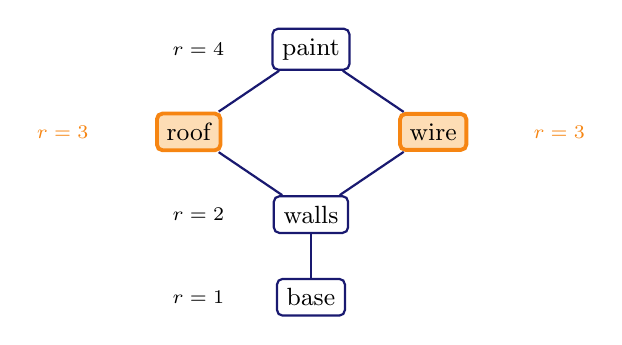
\begin{tikzpicture}[x=1.15cm,y=1.05cm,
  t/.style={draw=MidnightBlue,thick,rounded corners=2pt,fill=white,inner sep=3.5pt,font=\small},
  mid/.style={draw=BurntOrange,line width=1.4pt,rounded corners=2pt,fill=BurntOrange!25,inner sep=3.5pt,font=\small}]
  \node[t] (F) at (0,0) {base};
  \node[t] (W) at (0,1) {walls};
  \node[mid] (R) at (-1.35,2) {roof};
  \node[mid] (D) at (1.35,2) {wire};
  \node[t] (P) at (0,3) {paint};
  \draw[MidnightBlue,thick] (F) -- (W);
  \draw[MidnightBlue,thick] (W) -- (R);
  \draw[MidnightBlue,thick] (W) -- (D);
  \draw[MidnightBlue,thick] (R) -- (P);
  \draw[MidnightBlue,thick] (D) -- (P);
  \node[font=\scriptsize,anchor=east] at (-0.85,0) {$r=1$};
  \node[font=\scriptsize,anchor=east] at (-0.85,1) {$r=2$};
  \node[font=\scriptsize,BurntOrange,anchor=east] at (-2.35,2) {$r=3$};
  \node[font=\scriptsize,BurntOrange,anchor=west] at (2.35,2) {$r=3$};
  \node[font=\scriptsize,anchor=east] at (-0.85,3) {$r=4$};
\end{tikzpicture}
